%%%%%%%%%%%%%%%%%%%%%%%%%%%%%%%%%%%%%%%%%%%%%%%%%%%%%%%%%%%%%%%%
%                                                              %
%                                                              %
% Macallyster S. Edmondson                                     %
%                                                              %
% ECE351-53                                                    %
%                                                              %
% Lab #8                                                       %
%                                                              %
% 03/22/2022                                                   %
%                                                              %
% Straightforward layout, broken into sections, uses many      %
% common libraries. Note, Hyperlinks are not highlighted.      %
%                                                              %
%%%%%%%%%%%%%%%%%%%%%%%%%%%%%%%%%%%%%%%%%%%%%%%%%%%%%%%%%%%%%%%%

%%%%%%%%%%%%%%%%%%%%%%%%%%%%%%%%%%%%%%%%%%%
%%% DOCUMENT PREAMBLE %%%
\documentclass[12pt]{report}
\usepackage[english]{babel}
%\usepackage{natbib}
\usepackage{url}
\usepackage[utf8x]{inputenc}
\usepackage{amsmath}
\usepackage{graphicx}
\graphicspath{{./images/}}
\usepackage{parskip}
\usepackage{fancyhdr}
\usepackage{vmargin}
\usepackage{listings}
\usepackage[hidelinks]{hyperref}
\usepackage{xcolor}
\usepackage[nodayofweek]{datetime}
\usepackage[section]{placeins}
\usepackage{pdfpages}
\definecolor{codegreen}{rgb}{0,0.6,0}
\definecolor{codegray}{rgb}{0.5,0.5,0.5}
\definecolor{codeblue}{rgb}{0,0,0.95}
\definecolor{backcolour}{rgb}{0.95,0.95,0.92}
\lstdefinestyle{mystyle}{
backgroundcolor=\color{backcolour},
commentstyle=\color{codegreen},
keywordstyle=\color{codeblue},
numberstyle=\tiny\color{codegray},
stringstyle=\color{codegreen},
basicstyle=\ttfamily\footnotesize,
breakatwhitespace=false,
breaklines=true,
captionpos=b,
keepspaces=true,
numbers=left,
numbersep=5pt,
showspaces=false,
showstringspaces=false,
showtabs=false,
tabsize=2
}
\lstset{style=mystyle}
\setmarginsrb{3 cm}{2.5 cm}{3 cm}{2.5 cm}{1 cm}{1 cm}{1 cm}{1.5 cm}
\title{Lab \#8 Report}
% Title
\author{Macallyster S. Edmondson}
% Author
\newdate{date}{22}{03}{2022}
\date{\longdate\displaydate{date}}
% Date
\makeatletter
\let\thetitle\@title
\let\theauthor\@author
\let\thedate\@date
\makeatother
\pagestyle{fancy}
\fancyhf{}
\rhead{\theauthor}
\lhead{\thetitle}
\lfoot{Page: \thepage}
\rfoot{\thedate}
\fancypagestyle{customplain}{ %Used for default pages with plain style to keep overall document consistency
  \fancyhf{}
  \renewcommand{\headrulewidth}{0pt} %Remove bar from top of page
  \lfoot{Page: \thepage}
}
\fancypagestyle{titlepage}{ %Used for default pages with plain style to keep overall document consistency
  \fancyhf{}
  \renewcommand{\headrulewidth}{0pt} %Remove bar from top of page
  \cfoot{\thedate}
}
\fancypagestyle{customblank}{ %Used for default pages with plain style to keep overall document consistency
  \fancyhf{}
  \renewcommand{\headrulewidth}{0pt} %Remove bar from top of page
}
%%%%%%%%%%%%%%%%%%%%%%%%%%%%%%%%%%%%%%%%%%%%
\begin{document}
%%%%%%%%%%%%%%%%%%%%%%%%%%%%%%%%%%%%%%%%%%%%%%%%%%%%%%%%%%%%%%%%%%%%%%%%%%
%%%%%%%%%%%%%%%
\begin{titlepage}\thispagestyle{titlepage}
\centering
%\vspace*{0.5 cm}

\includegraphics[scale = 0.12]{univ-logo.png}\\[1.0 cm]
%University of Idaho
\begin{center}    \textsc{\Large   ECE 351 - Section \#53 }\\[2.0 cm]
\end{center}% University Name

%Lab Report
\rule{\linewidth}{0.2 mm} \\[0.4 cm]
{ \huge \bfseries \thetitle}\\
\rule{\linewidth}{0.2 mm} \\[0.5 cm]
\textsc{\Large Fourier Series Approximation of a Square Wave }\\[1.5 cm] % Course 
\begin{minipage}{0.4\textwidth}
\begin{flushleft} \large
\emph{Submitted To:}\\
Kate Antonov\\ \small
University of Idaho\\
kantonov@uidaho.edu\\
\hfill
\end{flushleft}
\end{minipage}~
\begin{minipage}{0.4\textwidth}
\begin{flushright} \large
\emph{Submitted By :} \\
\theauthor \\ \small
University of Idaho\\
edmo7033@vandals.uidaho.edu\\
\href{http://github.com/mac-edmondson}{github.com/mac-edmondson}\\
\end{flushright}
\end{minipage}\\[2 cm]
\vfill
\end{titlepage}
%%%%%%%%%%%%%%%%%%%%%%%%%%%%%%%%%%%%%%%%%%%%%%%%%%%%%%%%%%%%%%%%%%%%%%%%%%
%%%%%%%%%%%%%%%
\tableofcontents\thispagestyle{customplain}
\pagebreak
%%%%%%%%%%%%%%%%%%%%%%%%%%%%%%%%%%%%%%%%%%%%%%%%%%%%%%%%%%%%%%%%%%%%%%%%%%
%%%%%%%%%%%%%%%
\renewcommand{\thesection}{\arabic{section}}
\section{Introduction}
The goal of this weeks lab was to learn to approximate periodic time-domain signals with Fourier Series in Python, practicing using a basic Square Wave function. 
This lab was extremely helpful for my understanding of the related class topics. This lab was completed using \textit{Python} through the \textit{Spyder-IDE}. The 
packages used in the completion of this lab were \texttt{numpy} for definitions of mathematical functions and \texttt{matplotlib.pyplot} to plot outputs of functions.

All code for this lab, including this report, can be found on \href{http://github.com/mac-edmondson}{my Github}.
\section{Equations}\label{section: eq}
The equations used within this lab are shown in this section. The equations will be referenced by number throughout the rest of the report.

General Fourier Series Equations/Formulas:
\begin{equation}\label{eq: ffs} %Full Fourier Series
  \begin{aligned}[c]
    x(t) = \frac{1}{2}a_0 + \sum_{k=1}^{\infty}{a_k \cos(k\omega_0t) + b_k \sin(k\omega_0t)}
  \end{aligned}
\end{equation}
\begin{equation}\label{eq: ak}
  \begin{aligned}[c]
    a_k = \frac{2}{T} \int_0^T{x(t)\cos(k\omega_0t)dt}
  \end{aligned}
\end{equation}
\begin{equation}\label{eq: bk}
  \begin{aligned}[c]
    b_k = \frac{2}{T} \int_0^T{x(t)\sin(k\omega_0t)dt}
  \end{aligned}
\end{equation}
\begin{equation}\label{eq: w0}
  \begin{aligned}[c]
    w_0 = \frac{2\pi}{T}
  \end{aligned}
\end{equation}

Fourier Series found from preliminary:
\begin{equation}\label{eq: plfs} %prelab Fourier Series
  \begin{aligned}[c]
    x(t) = \sum_{k=1}^{N}{\frac{2}{k\pi}(1 - \cos(k \pi))\sin(k\omega_0t)}
  \end{aligned}
\end{equation}

\section{Methodology}
\subsection{Preliminary}\label{Section: Preliminary}
A crucial part of this lab was the preliminary work. Before the lab started, we found the Fourier Series approximation of the function seen in Figure \ref{fig: pre}.
Using Equations \eqref{eq: ffs}, \eqref{eq: ak}, \eqref{eq: bk}, and \eqref{eq: w0}, the Fourier Series approximation found is seen in Equation \eqref{eq: plfs}. 
My preliminary work can be found in the \nameref{section: Attachments} section of this report. Unfortunately, my first attempt at finding this approximation was 
a failure, but we covered the correct method during lab. Both methods used can be found in the attached work.

\begin{figure}[h!]
  \centering
  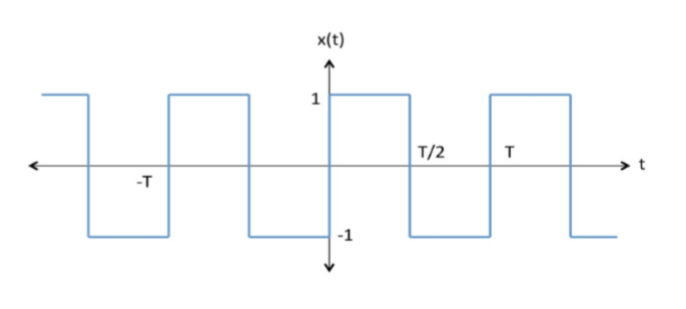
\includegraphics[scale=.7]{pre.png}
  \caption{Square Wave to Approximate}
  \label{fig: pre}
\end{figure}

\subsection{Lab: Part 1}\label{Section: Part1}
In Part 1 of this lab, the only part, we explored different approximations of the square wave function given in the lab handout (Figure \ref{fig: pre}) using the 
Fourier Series approximation found in the preliminary (Equation \eqref{eq: plfs}). 

We started by finding the first four values of $a_k$ \& $b_k$ after giving them function definitions. After this, we found the Fourier Series Approximation for
$N = \{1, 3, 15, 50, 150, 1500\}$. 

Below can be seen the code implementation of the tasks carried out in Part 1 of this lab.

\begin{lstlisting}[language=Python, basicstyle=\footnotesize]
#GLOBAL
step_size = 1e-3

# PART 1

#1
def b(k) :
    b_k = (2/(k*np.pi))*(1-np.cos(k*np.pi))
    return b_k

# a_k = 0; Thus is not defined.

print("a_k & b_k for 4 values.")
for i in range(1, 5, 1) :
    print("a_", i, "=", 0, " ; ", "b_", i, "=", b(i))

#2
T = 8;
w0 = 2*np.pi/T
def x(t, N) :
    x = 0
    for k in range(1, N+1, 1) :
        x += b(k) * np.sin(k*w0*t)
    return x

fList = [1, 3, 15, 50, 150, 1500]

for i in fList :
    t = np.arange(0, 20 + step_size, step_size)
    y1 = x(t, i)
    
    plt.figure(figsize = (10, 11))
    plt.subplot(1, 1, 1)
    plt.plot(t, y1, "b-")
    plt.grid()
    plt.ylabel('x(t) [N = ' + str(i) + ']')
    plt.xlabel('t')
    plt.title(Fourier Series Output for N = ' + str(i))
\end{lstlisting}

\section{Results}\label{section: Results}
The results of this lab are very straightforward. The implementation of all functions worked as expected and the results are as expected.

The deliverables for Part 1 of this lab are seen in all figures given below. As can be seen in all graphs, as N increases the approximation of the function 
gets better. This explains why in the definition of the Fourier Series as $N\to\infty$, the desired function should be perfectly approximated.
\\
\begin{figure}[h!]
  \centering
  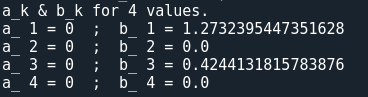
\includegraphics[scale=1]{p1t1.png}
  \caption{First Four Terms of Fourier coefficients ($a_k$ \& $b_k$)}
  \label{fig: p1t1}
\end{figure}
\begin{figure}[h!]
  \centering
  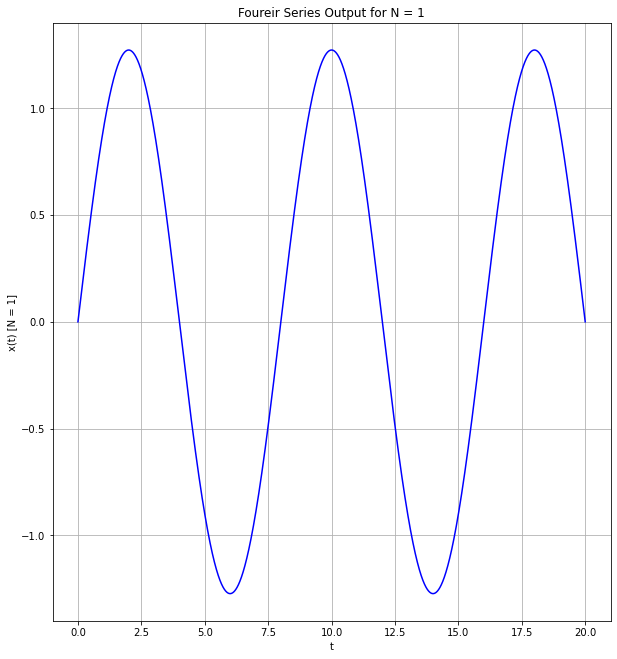
\includegraphics[scale=.5]{p1t2-0.png}
  \caption{Fourier Approximation for $N = 1$}
  \label{fig: p1t2-0}
\end{figure}
\begin{figure}[h!]
  \centering
  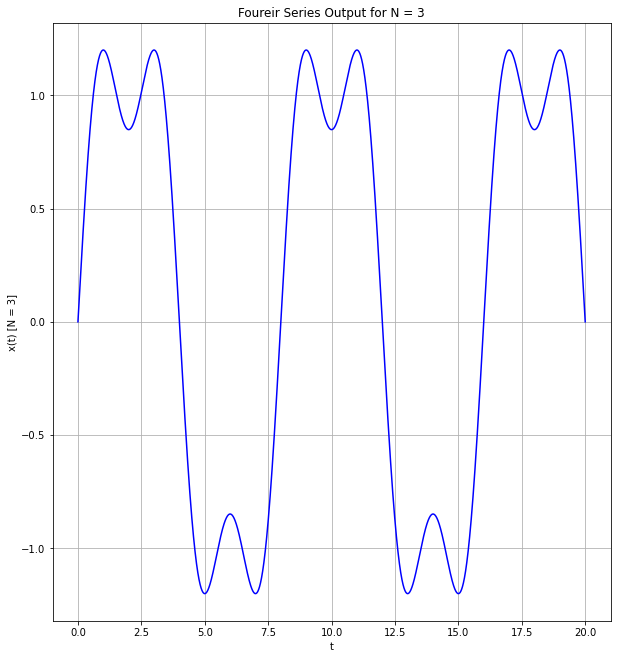
\includegraphics[scale=.5]{p1t2-1.png}
  \caption{Fourier Approximation for $N = 3$}
  \label{fig: p1t2-1}
\end{figure}
\begin{figure}[h!]
  \centering
  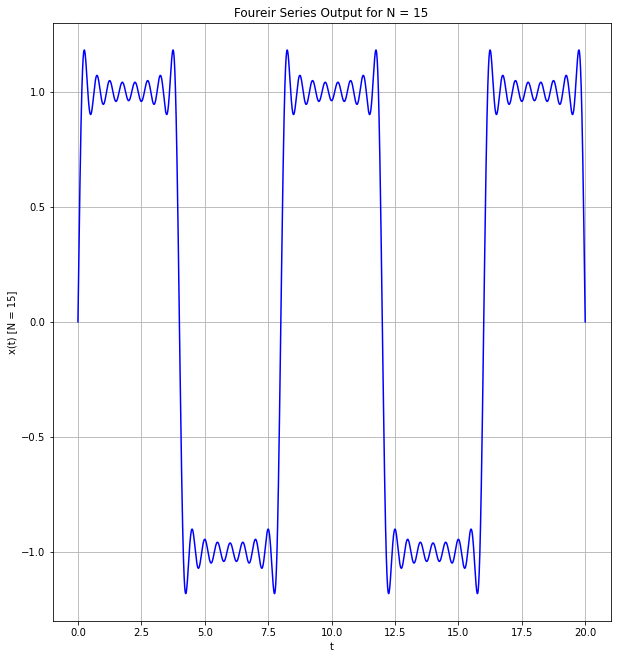
\includegraphics[scale=.5]{p1t2-2.png}
  \caption{Fourier Approximation for $N = 15$}
  \label{fig: p1t2-2}
\end{figure}
\begin{figure}[h!]
  \centering
  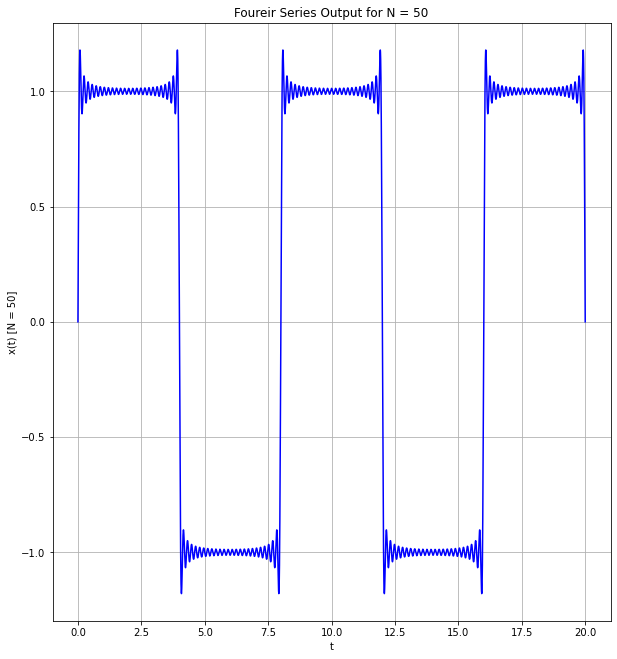
\includegraphics[scale=.5]{p1t2-3.png}
  \caption{Fourier Approximation for $N = 50$}
  \label{fig: p1t2-3}
\end{figure}
\begin{figure}[h!]
  \centering
  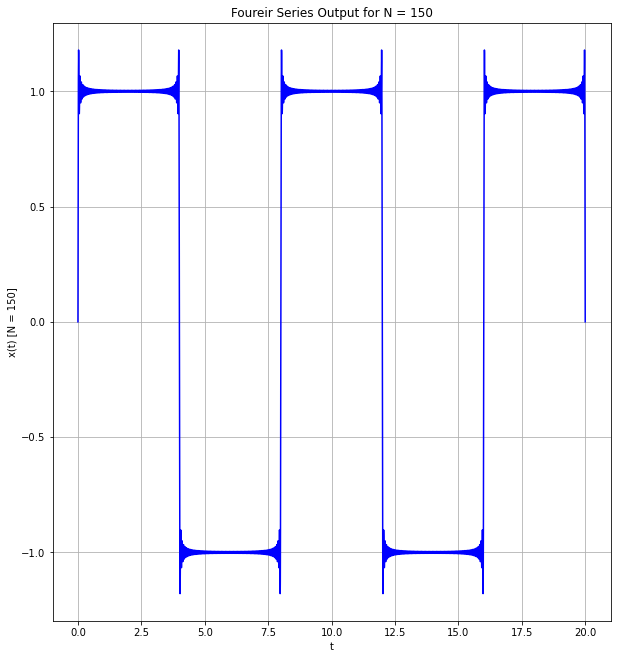
\includegraphics[scale=.5]{p1t2-4.png}
  \caption{Fourier Approximation for $N = 150$}
  \label{fig: p1t2-4}
\end{figure}
\begin{figure}[h!]
  \centering
  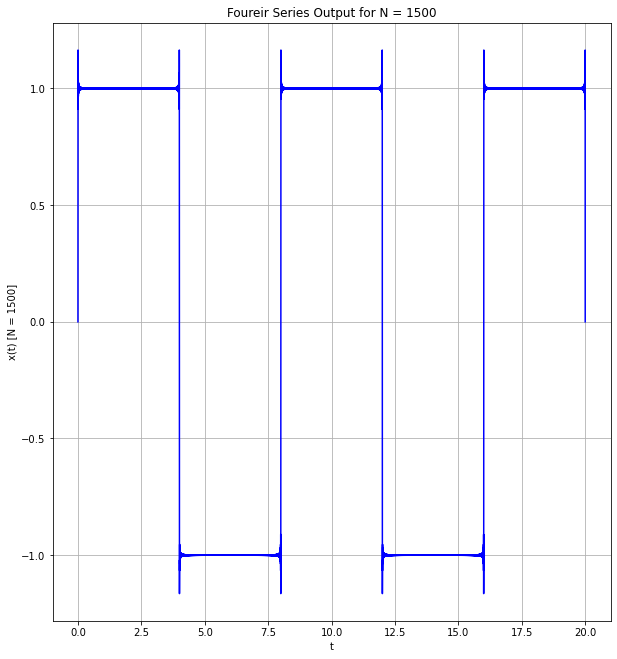
\includegraphics[scale=.5]{p1t2-5.png}
  \caption{Fourier Approximation for $N = 1500$}
  \label{fig: p1t2-5}
\end{figure}
\section{Error Analysis}\label{section: ErAn}
No sources of error were seen throughout this lab, and I did not run into any real problems while implementing anything lab lab asked. The implementation of 
Task 2 of this lab took some time to implement properly, but as seen from \nameref{Section: Part1} the code is not that complicated to 
understand.
\section{Questions}
\begin{enumerate}
  \item In Figure \ref{fig: pre}, the square wave function seen is odd as $f(-x)=-f(x)$.
  \item As seen from the preliminary in \nameref{section: Attachments}, the values of $a_2, a_3, ... , a_n$ do not really matter as the term associated with that
  coefficient will go to zero.
  \item As seen in the \nameref{section: Results} section of this report, as N increases the better the approximation of the Square wave becomes. With only 1500
  terms, the approximation looks pretty good but is far from perfect. As seen in majority of Fourier Series, there is a ringing at the peak edges of the square
  wave which is the biggest visual difference in the approximation.
  \item Mathematically, as the value of N increases more terms of monotonically increasing harmonics are added to the series. This further fills the inaccuracies
  of the current approximation and leaves you with a better looking approximation as $N\to\infty$.
  \item Purpose, deliverables, and expectations were very clear for this lab.
\end{enumerate}
\section{Conclusion}
In conclusion, I feel this lab was very successful. The implementation of the code in this lab was quite simple and I really enjoyed seeing how you could
find the total transfer function with some symbolic math and Python. All in all, I am very satisfied with what this lab has taught me and feel it was an 
excellent use of time.
\newpage
\thispagestyle{customblank}
\section{Attachments}\label{section: Attachments}
% No attachments for this lab.
\centering\begin{enumerate}
  \item Pre-Lab
\end{enumerate}
\vspace*{\fill}

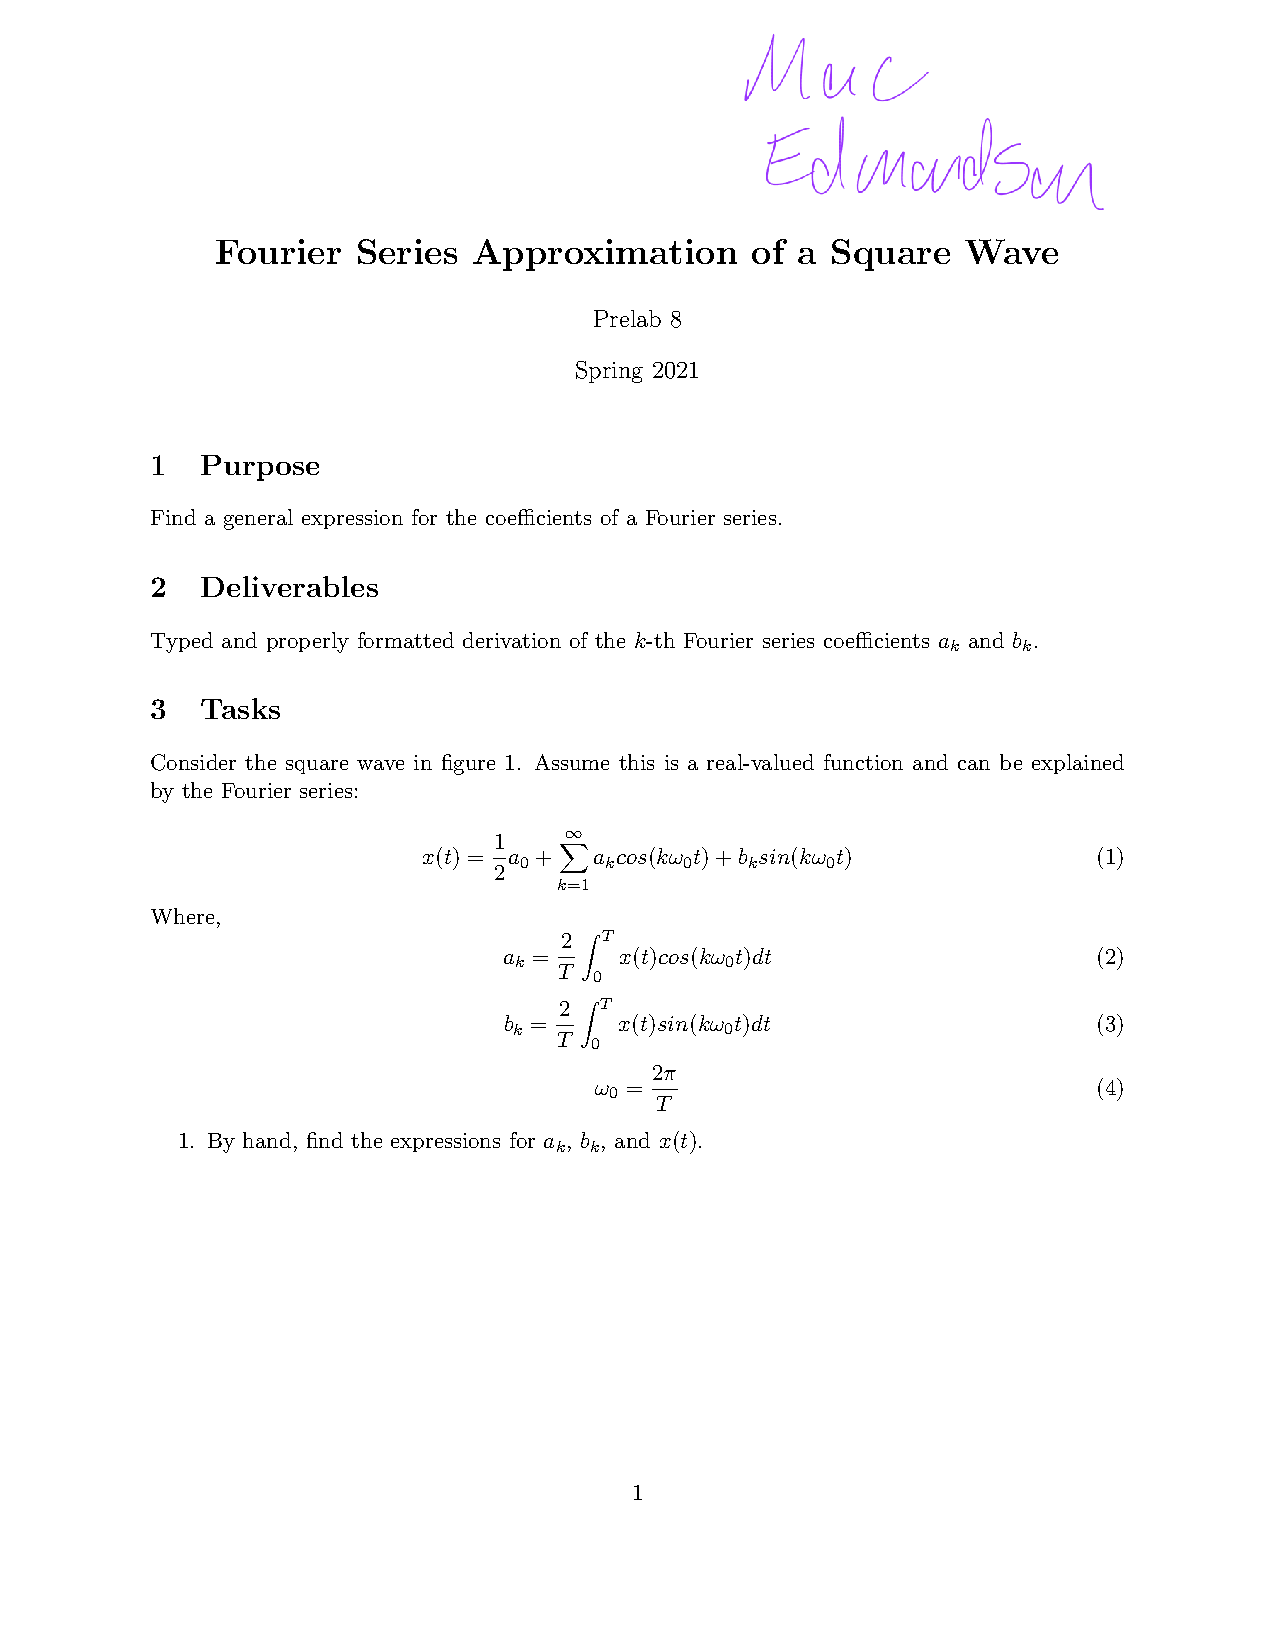
\includepdf[pages=-, offset=1in -1in]{./attachments/lab8_pre.pdf}
% \includepdf[pages=3, offset=1in -1in]{./attachments/lab5.pdf}

% \begin{thebibliography}{111} 
% \thispagestyle{customplain}

% \end{thebibliography}
\end{document}
%This template was created by Roza Aceska.